\documentclass[12pt,oneside,letterpaper]{article}

\usepackage{ASEE_Settings}

\begin{document}

    \pagenumbering{roman} 
    \begin{center}

    \vspace*{-2cm} % Adjust this value to move the content up
    {\fontsize{14pt}{17pt}\selectfont\bfseries Student Paper} \\
    {\fontsize{14pt}{17pt}\selectfont\bfseries Work in Progress: High Altitude Robotic Monkey} \\

\end{center}

    \addcontentsline{toc}{section}{Abstract}
    \textbf{Abstract} - This Work In Progress paper is about a high altitude ballooning payload involving long distance robotics communications. In 2018, as part of a NASA-funded student project, undergraduate students developed a robotic monkey which successfully operated on a 2000-gram high-altitude balloon (HAB) and flew to an altitude of 4,000 feet and a range of 12 miles. The robot, named HAM (for “High Altitude Monkey”), moves, speaks, and broadcasts live video while in flight. Its purpose was to interact with K-12 students on the ground as an educational tool to teach “Near Space” science. That robot is now part of the university’s mobile laboratory (STEM bus), which travels to local area schools and community events around the state, promoting near space research and STEM education.

In the academic year 2024-2025, a new group of interdisciplinary engineering and computer science students will build an enhanced robot and resume its high-altitude ballooning flights. A major enhancement to the robot’s flight control payload is the addition of a controllable and autonomous vent. The vent is attached to the high-altitude balloon itself and can be opened or closed to release helium, allowing the balloon to remain at a specified altitude and enabling altitude-controlled termination of the flight. Additionally, the vent system will enable the payload to stay near the ground station site, supporting better live stream transmission and reception.

The target for this project is to launch HAM to 15,000 feet and travel approximately 20 miles while maintaining a direct live feed for the entire flight. A team of undergraduate and graduate students will have the opportunity to perform fundamental research in developing this payload. The successful completion of HAM will support the use of robotics in near-space applications as well as research on long-distance communications and transmissions. The outcomes from this project will be disseminated through demonstrations on the university’s mobile laboratory for K-12 students and through peer-reviewed publications.
    
\textbf{Keywords}

    high-altitude, balllooning, robotics

 
    
    %\newpage
    %\addcontentsline{toc}{section}{Acknowledgments}
    %Insert Acknowledgments here

\begin{comment}
    \newpage
    \doublespacing
    \addcontentsline{toc}{section}{Table of Contents}
    \renewcommand{\baselinestretch}{1}\normalsize
    \tableofcontents
    \renewcommand{\baselinestretch}{1}\normalsize
    \singlespacing
    \thispagestyle{fancy} % force page style
\end{comment}    
    %\newpage
    %\pagenumbering{arabic} 
    %\fancyfoot[C]{Page \thepage\ of \pageref{EndOfText}} 
    % We can change \pageref{endOfDoc}} back to \...{EndOfText}
    % once we have more things to append to the end
    % TODO: Check below for other notes
    %\newpage
    \setlength{\parskip}{\baselineskip} % Blank line between paragraphs
    \label{ch1}
    \section{Introduction}
\vspace{-2em}

High-altitude ballooning has long served as an inexpensive flight platform for testing remote sensing instrumentation for Earth and space applications, communication systems, and other spaceflight hardware, offering quick turnaround and operational flexibility~\cite{HAB_Fundamentals}. The versatility of a high-altitude balloon flight provides a multidisciplinary platform for experiential learning, enabling students to design and execute a wide range of experiments shaped by both educational objectives and technical constraints. \par

%, as seen in Figure~\ref{Fig:HAB_Flight}

\begin{comment}
\begin{figure}[H]
    \centering
    \includegraphics[width = 0.7\textwidth]{Figures/HAM_Wiring_Comparison.jpg}
    \caption{High Altitude Ballooning Flight}
    \label{Fig:HAB_Flight}
\end{figure}
\vspace{-2em}  % Reduce space after the figure
\end{comment}

HAM (an acronym for High Altitude Monkey) was developed by undergraduate students at the University of Bridgeport in 2015 as part of their fulfillment of the Bachelor of Science degree requirements in Electrical Engineering and Computer Science. The payload was named in homage to Ham, the first chimpanzee to travel into space aboard the Mercury-Redstone 2 mission in 1961, a historic milestone in human spaceflight~\cite{Burgess2014}. 

\begin{figure}[H]
    \centering
    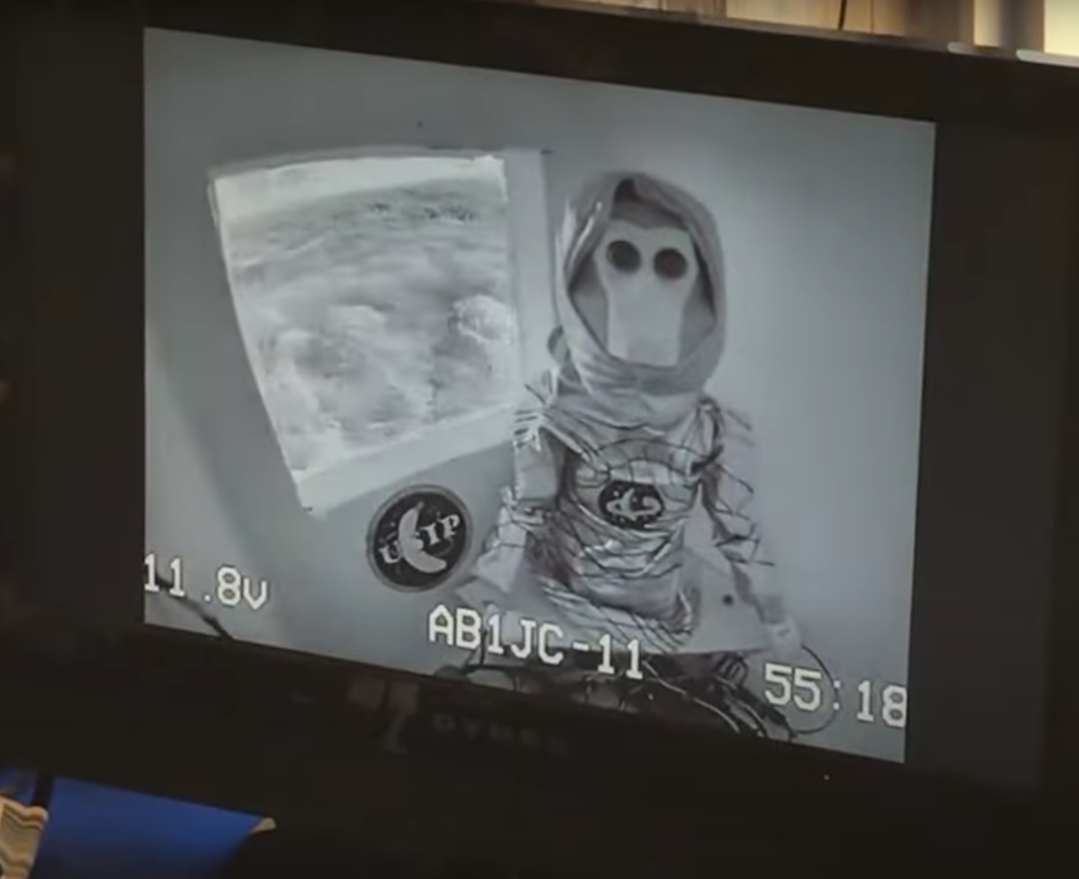
\includegraphics[width = 0.6\textwidth]{Figures/HAM_Original_Flight.png}
    \caption{Still image from HAM’s maiden launch in November 2019}
    \label{Fig:HAB_2019_Flight}
\end{figure}
\vspace{-2em}  % Reduce space after the figure
Weighing just under 12 pounds, HAM completed its maiden flight in November 2019 over Bridgeport, Connecticut, where the payload was used to engage attendees at a local children's museum during a special outreach event. Figure~\ref{Fig:HAB_2019_Flight} shows HAM successfully establishing communication at an altitude of 500 feet, transmitting telemetry data and receiving movement commands in real time. The flight traveled approximately 14 miles east, reaching a peak altitude of 4,000 feet before landing on a beach in Milford, Connecticut. \par

In the 2024–2025 academic year, students in the Extreme Environments Laboratory aim to conduct a second flight using a redesigned model of HAM, incorporating nearly a decade of technological advancements. This study outlines the steps taken to improve HAM's 3D modeling and wiring, with the goal of enhancing the payload's efficiency and reducing its weight. It also explores potential design modifications and broader applications of HAM in future high-altitude ballooning missions.

\vspace{-2em}
\section{Structure and Subsystems}
\vspace{-2em}

This system is designed to utilize amateur radio frequencies for data transmission and is capable of operating at altitudes up to 10{,}000~feet (approximately 3~kilometers). The 2019 flight system consisted of two primary components: (1) an onboard telemetry and communications payload employing a TinyTrak4 module from Byonics~\cite{byonics_tinytrak4}, and (2) the main visual payload, shown in Figure~\ref{Fig:HAB_2015_Inside}, which transmitted black-and-white video signals over amateur radio frequencies. Data packets were transmitted and received using the Automatic Packet Reporting System (APRS), enabling real-time interpretation and display at the ground command center, as illustrated in Figure~\ref{Fig:HAB_2015_Command}. From this station, children were able to interact with HAM live during the mission. Commands sent from the ground were received by the telemetry payload and relayed to the visual payload via a local Bluetooth network using HC-05 modules. After executing the command, the telemetry system transmitted confirmation back to the ground, enabling the next command to be issued.

\begin{figure}[H]
    \centering
    \begin{subfigure}[t]{0.49\textwidth}
        \centering
        \includegraphics[width=\textwidth, angle=-90]{Figures/HAM_Original.JPG}
        \caption{Internal view of primary robotics payload}
        \label{Fig:HAB_2015_Inside}
    \end{subfigure}
    \hfill
    \begin{subfigure}[t]{0.49\textwidth}
        \centering
        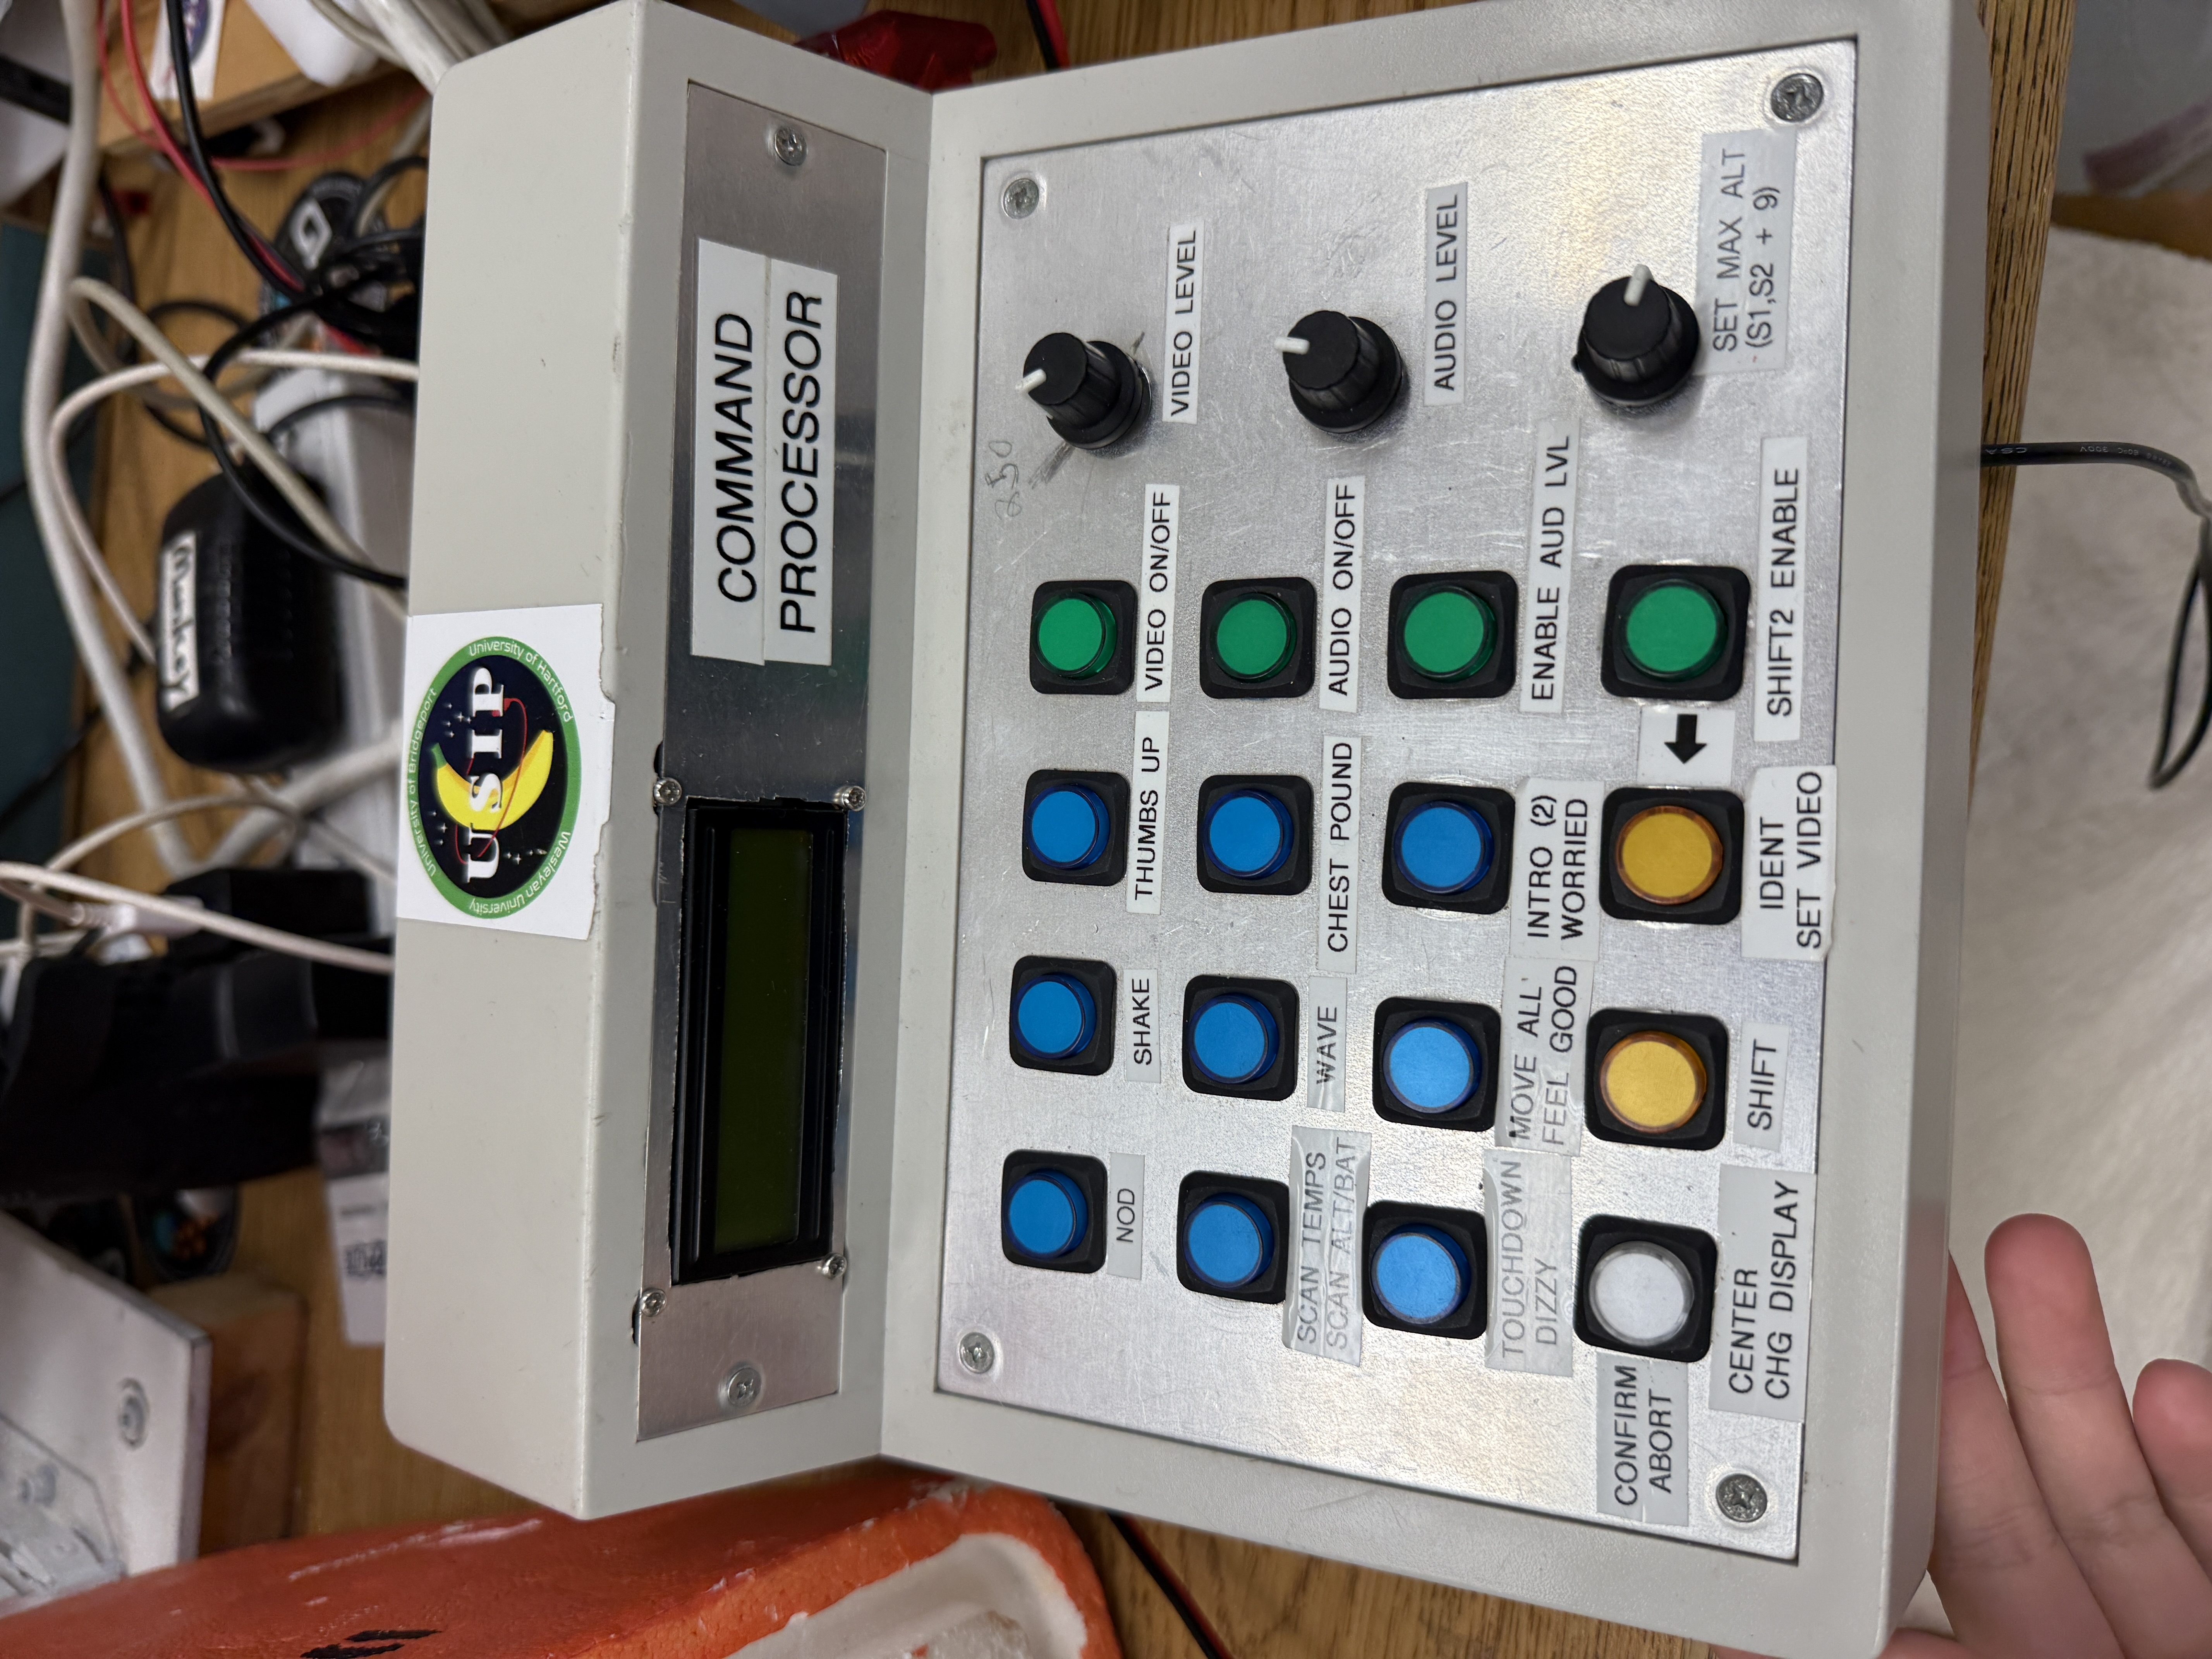
\includegraphics[width=\textwidth, angle=-90]{Figures/Command_Processor.JPG}
        \caption{Command processing unit}
        \label{Fig:HAB_2015_Command}
    \end{subfigure}
    \caption{Overview of HAM's 2015 internal components and control systems configuration}
    \label{Fig:HAB_2015_Combined}
\end{figure}
\vspace{-2em}

The updated configuration will feature streamlined circuitry through printed circuit boards (PCBs), along with a reduction in overall payload weight. Additional upgrades include dual GPS tracking systems for improved accuracy and redundancy, an onboard venting system for precise control of ascent and descent, a cut-down mechanism for safe recovery, and a 360\degree{} camera to document HAM’s flight and enhance operational safety. \par

The research conducted in this project is highly novel within the field of high-altitude ballooning. Most flight systems rely on static payloads that primarily transmit data to the ground, without incorporating mechanical motion or interactive components. HAM distinguishes itself as a unique innovation by integrating constant bidirectional communication, moving mechanisms, and real-time telemetry, all streamed to the ground via live video feed. \par 
    
    %\newpage
    \label{ch2}
    %\subsection{What has been accomplished?  What additional work needs to be done?}

\vspace{-2em}  % Reduce space after the figure
\section{Methodology}
\vspace{-2em}  % Reduce space after the figure

In the new iteration of HAM, numerous optimizations have been identified following nearly a decade of technological advancement. While improvements in circuitry and power delivery were a primary focus, several components from the original system had become outdated or obsolete, necessitating the selection and programming of modern replacements. To initiate the redesign process, students reviewed the original HAM project documentation, which outlined core components and movement logic. Gudi collaborated with members of the HAM (2015) team to draft an updated parts list, while Huong began analyzing the original mechanical systems and developing a comprehensive digital schematic for all pin connections. \par

\vspace{-2em}  % Reduce space after the figure
\section{Printed Circuit Boards}
\vspace{-2em}  % Reduce space after the figure

On the 2015 iteration of the project, HAM relied on a breadboard and jumper wires to connect all necessary components. While the system functioned as intended during flight, it posed challenges for post-flight maintenance and troubleshooting. In the 2025 iteration, HAM transitioned to using dedicated printed circuit boards (PCBs) for all subsystems. This shift improved modularity, simplified component replacement, and enabled systematic documentation for future development. \par

The system was divided into four PCBs, each serving a specific function: (1) the primary flight payload, (2) telemetry transmission, (3) video processing, and (4) mission control interface. Adopting PCBs not only streamlined the internal layout but also eliminated the bulk and complexity of breadboard wiring, resulting in a 10\% reduction in overall payload weight, as shown in Figure~\ref{Fig:Wiring_SideBySide}. \par

\begin{figure}[H]
    \centering
    \includegraphics[width=0.8\textwidth]{Figures/HAM_Wiring_Comparison.jpg}
    \caption{Side by side comparison of circuitry}
    \label{Fig:Wiring_SideBySide}
\end{figure}
\vspace{-2em}

These circuit boards incorporate design improvements that significantly enhance maintainability. Major upgrades include:

\vspace{-2em}
\begin{itemize}
    \item Dual power inputs (Anderson and 2.1~mm barrel jack) to accommodate both flight and ground configurations, replacing the previous setup of multiple Anderson connectors
    \item Integrated on/off power switch for streamlined testing and controlled power cycling
    \item Compact-form-factor ATmega2560 microcontroller for embedded control, replacing the larger Arduino Mega 2560 Rev 3
    \item Surface-mountable 1206 chip resistors, replacing legacy through-hole metal film resistors
    \item Modular hardware layout enabling easy component replacement and system reconfiguration
\end{itemize}

These improvements not only reduce the overall payload weight but also enhance the system’s reliability during both flight and testing. By transitioning to a more modular and compact design, the updated boards streamline troubleshooting and future development efforts. As a result, the HAM system is now better equipped to support extended missions and iterative upgrades across future launch campaigns.

\vspace{-2em}  % Reduce space after the figure
\section{Model Optimization}
\vspace{-2em}  % Reduce space after the figure

The original HAM model was 3D printed using PLA and designed to accommodate six servo motors. With a total weight of 15.4 ounces, the team identified the torso—accounting for 5 ounces—as a key target for weight reduction in future revisions. According to FAA guidelines, total payload stacks must not exceed a 12-pound weight limit~\cite{CFR_Part_101}; therefore, every ounce becomes critical at launch.

\begin{figure}[H]
    \centering
    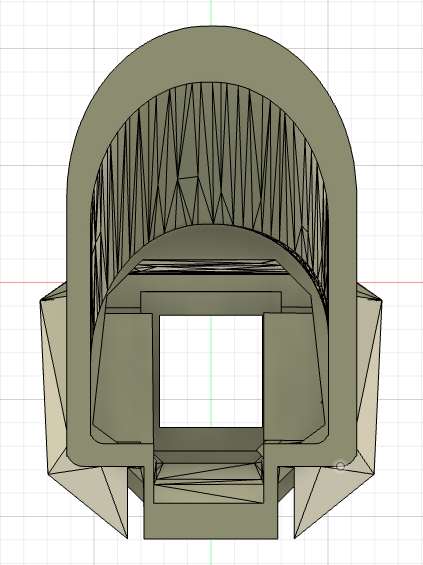
\includegraphics[width=0.24 \textwidth]{Figures/Model_Bottom_View.png}
    \caption{Bottom view of the updated Torso model}
    \label{Fig:Model_Bottom}
\end{figure}
\vspace{-2em}

The redesigned torso was split into two separate pieces to reduce the need for support material and improve print efficiency. This modular approach also simplifies maintenance, allowing for individual sections to be replaced without disassembling the entire body. Additionally, the internal structure was hollowed to minimize material usage, reducing the torso weight to 3.8 ounces. With all six servo motors installed, the complete model now weighs 11.9 ounces—an overall improvement of 22\% compared to the original design. \par

\vspace{-2em}  % Reduce space after the figure
\section{Additional Payloads}
\vspace{-2em}  % Reduce space after the figure

Alongside HAM’s telemetry and live-streaming systems, the overall flight stack will also include a dedicated communications payload to establish bidirectional data transfer between the flight system and the ground station. This will ensure reliable transmission of real-time telemetry during ascent and descent. Additionally,  we plan to integrate three supplementary payloads: (1) a 5.7k resolution 360° camera for flight documentation, (2) a SPOT Trace GPS tracker for redundancy in tracking and recovery, and (3) a venting system to regulate internal pressure and temperature of the balloon. These components were core elements of the University’s contributions to the Nationwide Eclipse Ballooning Project from 2022 to 2024 \cite{NEBP_Website}.
    
    %\newpage
    \label{ch3}
    \vspace{-2em}
\section{Result \& Discussion}
\vspace{-2em}

The preliminary findings from this research reflect not only strong technical progress toward a successful flight in June 2025, but also highlight the educational impact of interdisciplinary skill-building and the broader outreach potential of HAM as an interactive STEM platform.

To date, students have successfully established APRS communication with the payload at distances of 20 and 200 feet, verifying baseline functionality between the visual payload, telemetry, and APRS. The system continues to perform reliably and remains on track for full integration by the end of May 2025. Additional validation through a preliminary tethered launch is planned to assess data transmission capabilities under simulated flight conditions.

Notably, neither of HAM’s lead students comes from a traditional background in mechanical or electrical engineering—disciplines upon which this renovation heavily relies. Despite this, both Huong and Gudi, having previously participated in high-altitude ballooning missions, earned their degrees in Computer Science and took the initiative to independently acquire the interdisciplinary skills required for this project. These skills span soldering, 3D modeling, schematic design, PCB layout, and project management. Their technical contributions have been instrumental to the project’s success and have significantly enriched their academic growth and professional readiness as they prepare to enter industry roles.

Unlike many ballooning payloads that operate passively with minimal engagement, HAM introduces a unique interactive component. By responding to real-time commands during flight, HAM creates opportunities for live engagement with students and observers on the ground. This interactivity enables us to teach foundational STEM principles—such as robotics, telemetry, and embedded systems—to learners of all ages via our STEM on Wheels program, the University's mobile STEM laboratory. Just as the original HAM the Chimpanzee inspired a generation in 1961 \cite{Burgess2014}, our goal is for this modern-day HAM to spark curiosity and inspire the next generation of scientists and engineers through meaningful, hands-on experiences.
    
    %\newpage
    \label{ch4}
    \vspace{-2em}
\section{Future Outlooks and Considerations}
\vspace{-2em}

High-altitude ballooning has enabled researchers to conduct iterative experiments with rapid turnaround, offering a flexible and cost-effective alternative to traditional astronomical research. HAM was originally designed to engage K–12 students through interactive, hands-on science experiences, and our team is committed to continuing this mission. Through the University of Bridgeport's \textit{STEM on Wheels} program—a mobile laboratory that brings STEM activities directly to schools across Connecticut—we aim to inspire students and educators by demonstrating real-world applications of science and engineering.

To further encourage adoption and innovation, all design files and documentation for HAM will be made publicly available via GitHub. This will allow other institutions to replicate our work, build their own high-altitude flight companions, and contribute to a growing community focused on improving communication systems in unmanned stratospheric flights.

The success of the HAM project is the result of contributions from students, faculty, and alumni spanning multiple generations and disciplines. Looking ahead, the university plans to establish HAM as an annual project embedded within intercollegiate clubs—providing interdisciplinary teams of undergraduate and graduate students with the opportunity to apply their skills and propose system-level improvements. Areas currently under review for future revisions include:

\vspace{-2em}
\begin{itemize}
    \item Integration of DC-DC power conversion units and reconfiguration of power distribution systems
    \item Use of the ATmega2560 microcontroller with a direct programming and communication interface
    \item Replacement of proprietary communication modules with onboard Bluetooth
    \item Substitution of the discontinued EMIC 2 Text-to-Speech module with a modern alternative
    \item Enhancement of servo motor performance through the integration of Bottango software for unique "Monkey-like" motions \cite{Bottango}
\end{itemize}
\vspace{-2em}

This High Altitude Robotic Monkey exemplifies the power of interdisciplinary learning, hands-on engineering, and public outreach through high-altitude ballooning. From its roots as a student-driven initiative to its evolution into an interactive STEM platform, HAM has provided valuable educational experiences, technical challenges, and outreach opportunities. As the project concludes its 2025 iteration, it lays the foundation for continued development, regular deployment, and broader adoption by academic institutions seeking to engage students in space-related research. With open-source documentation, long-term university support, and integration into community outreach, HAM is positioned to serve as both a model for experiential learning and a catalyst for future innovation in stratospheric flight.
    
    \label{EndOfText}
    
    \newpage
    %\pagenumbering{Roman} 
    %\addcontentsline{toc}{section}{References}
    %\fancyfoot[C]{Page \thepage\ of \pageref{EndOfDoc}}
        \nocite{*}
        \footnotesize{\bibliographystyle{unsrt}\bibliography{Bibliography}}
        %\thispagestyle{fancy}
    
    %\newpage
    %\addcontentsline{toc}{section}{List of Figures}
    %\listoffigures
    %\thispagestyle{fancy}
    
    %\newpage
    %\addcontentsline{toc}{section}{List of Tables}
    %\listoftables
    %\thispagestyle{fancy}
    \label{EndOfDoc}
\end{document}